\section{Results}

- microbenchmarks: fio randread/write, vary bs, qd, 
- filebench

- compare lsvd/rbd
- theoretical upper limit with local nvme

- latency histograms? bimodal of hit/miss should show up somewhere
- vm boot results
- image optimization

Notes on figures themselves:

- Separate by workload instead of config 
  -- ex one fileserver graph with all the configs instead of multiple with fileserver 


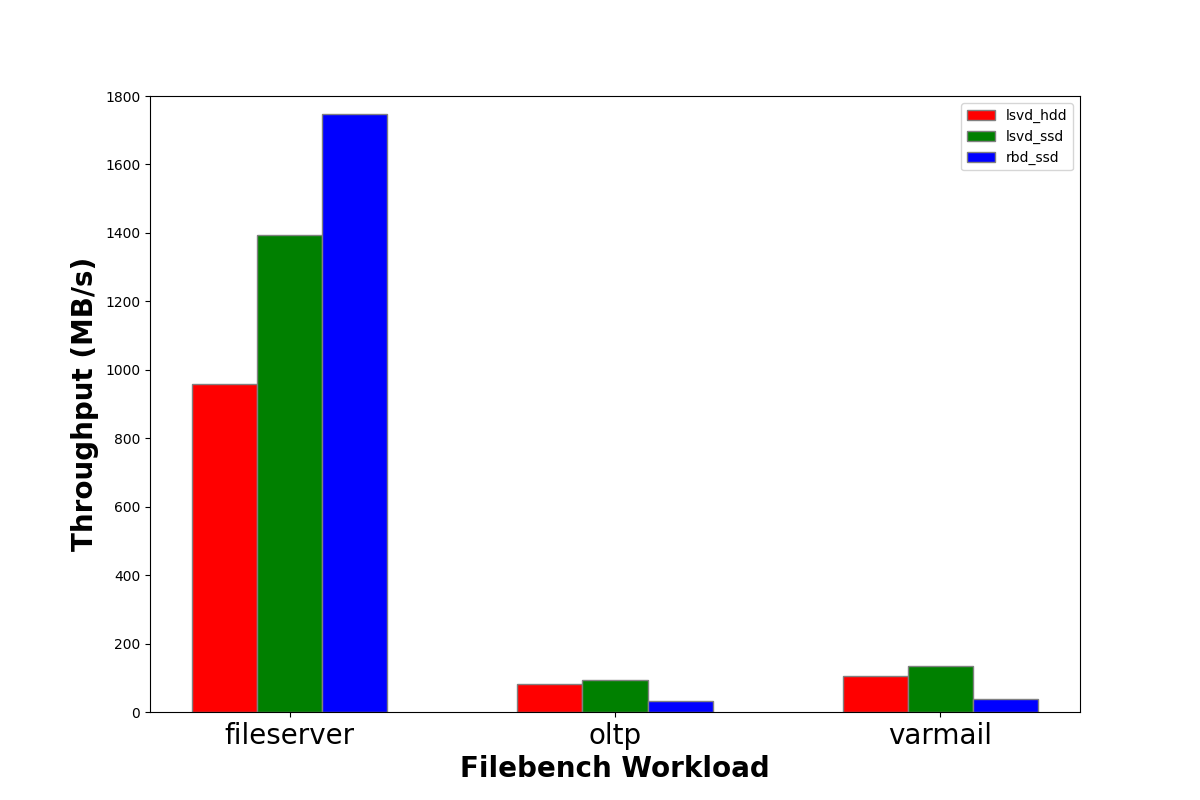
\includegraphics[width=8cm, height=6cm]{graphs/filebench_20g.png}
Fig1. File benchmark result with 20GB Cache and 80GB Volume. 

- The hdd with lsvd is comparable to rbd and lsvd with ssd


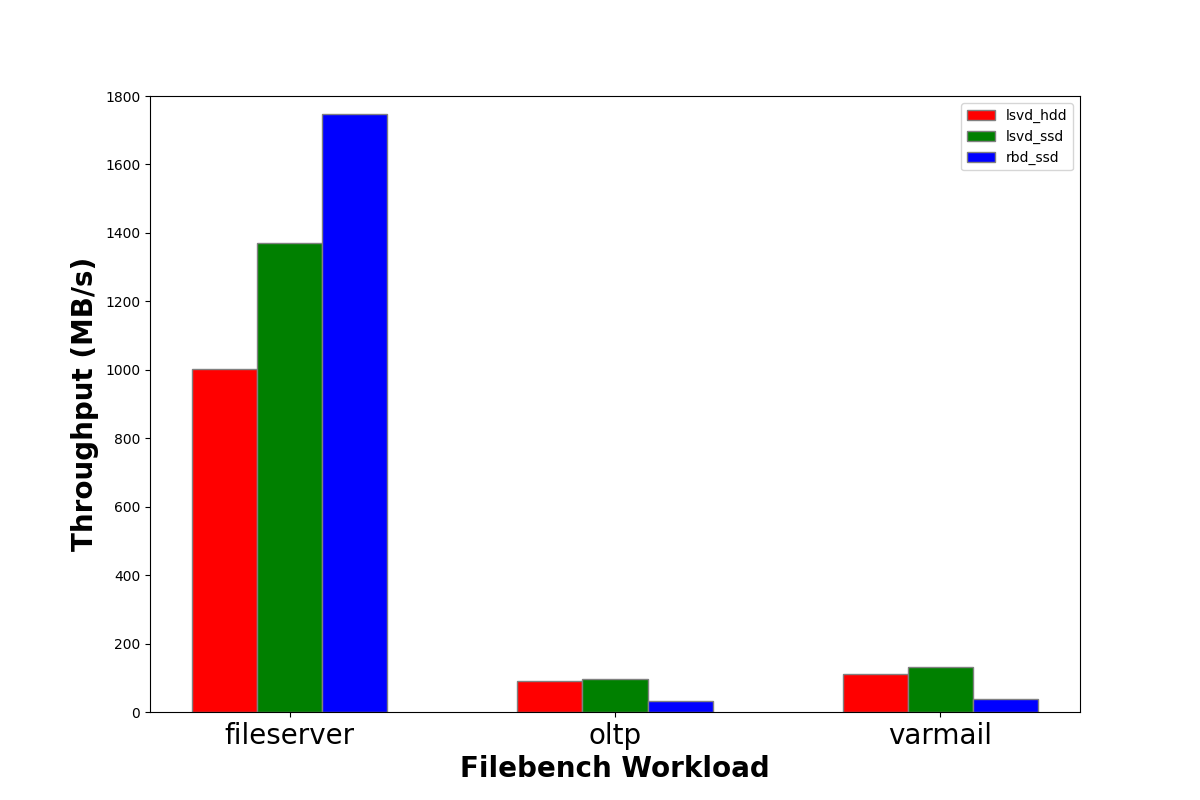
\includegraphics[width=8cm, height=6cm]{graphs/filebench_240g.png}
Fig2. File benchmark result with 240GB Cache and 80GB Volume.

- The result is similar to small cache (should we keep both?)

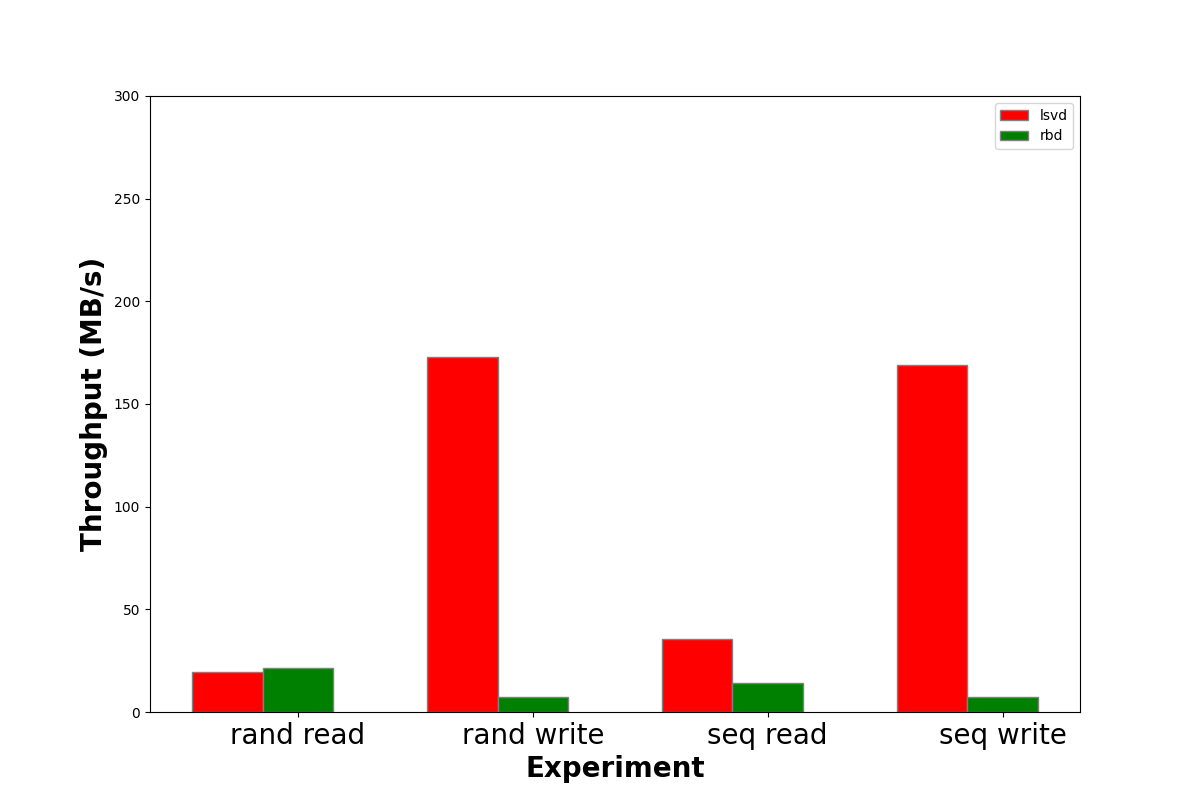
\includegraphics[width=8cm, height=6cm]{graphs/request_bw_hdd_20gb.png}
Fig3. Micro benchmark result with 20GB Cache, 80GB Volume and Hard Disk Backend.


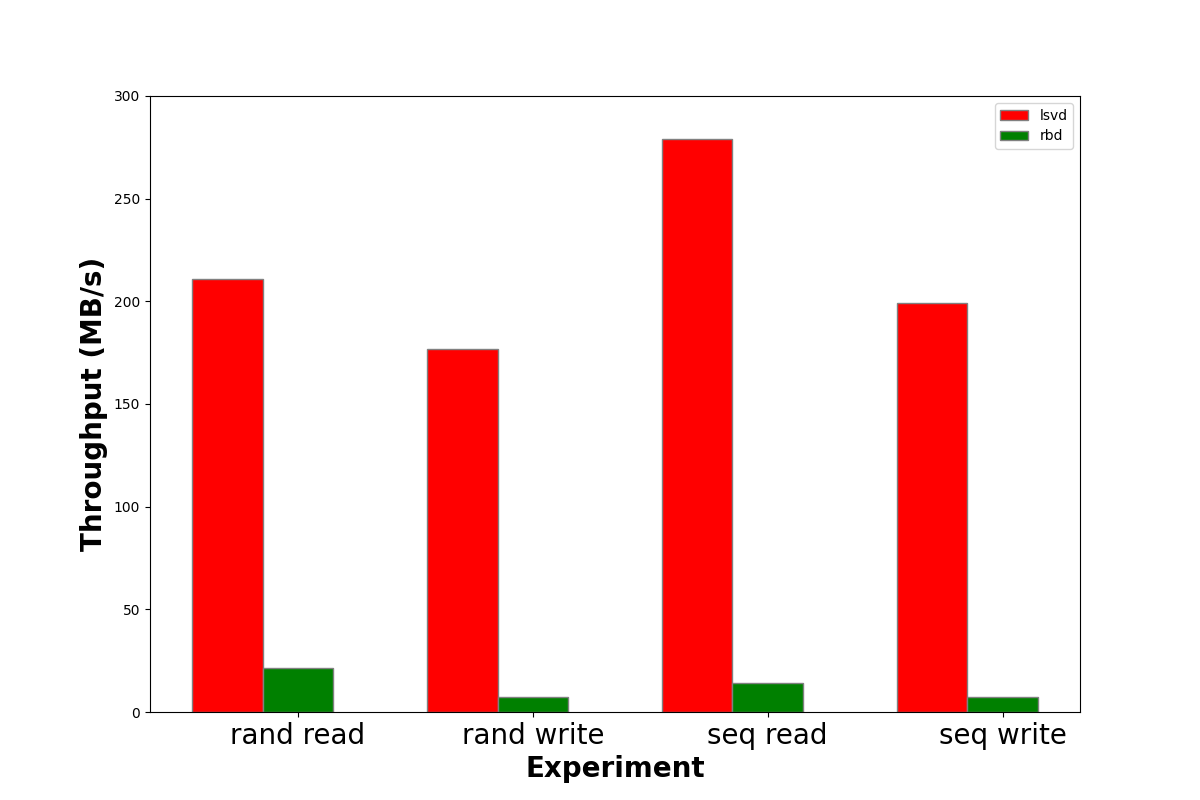
\includegraphics[width=8cm, height=6cm]{graphs/request_bw_hdd_240gb.png}
Fig4. Micro benchmark result with 240GB Cache, 80GB Volume and Hard Disk Backend.


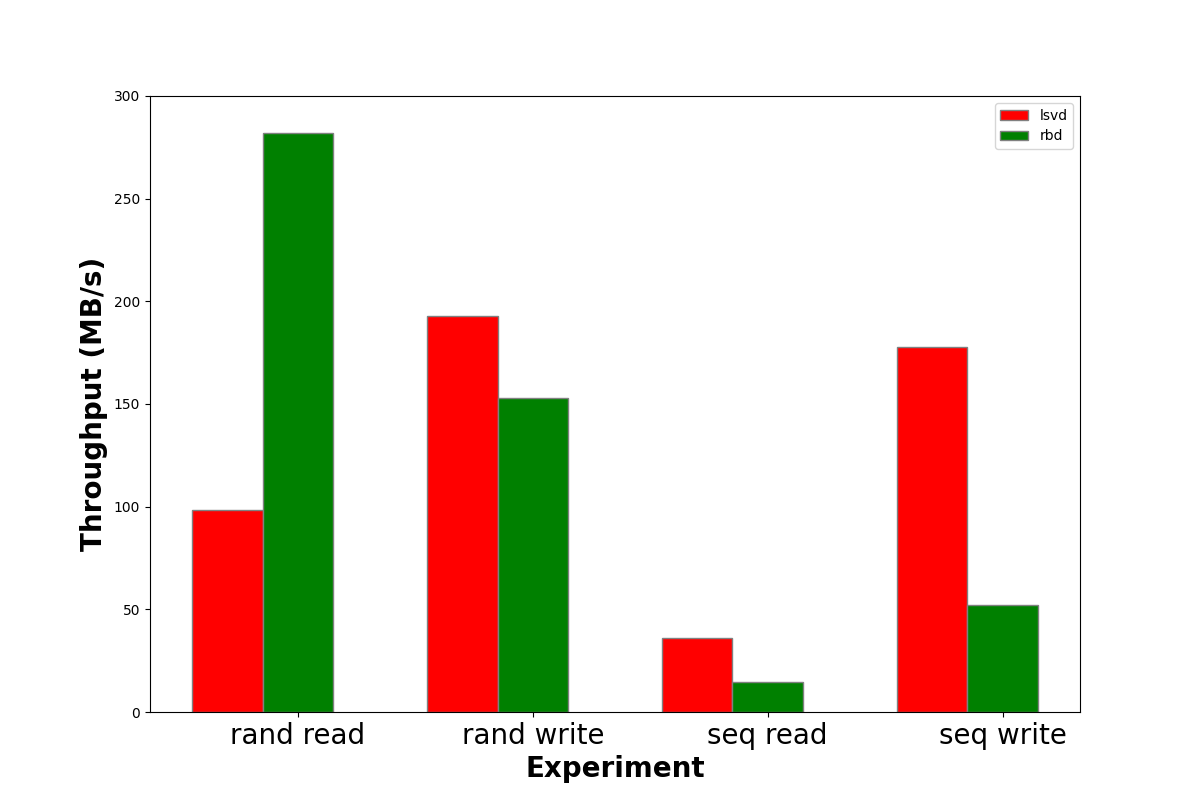
\includegraphics[width=8cm, height=6cm]{graphs/request_bw_ssd_20gb.png}
Fig5. Micro benchmark result with 240GB Cache, 80GB Volume and SSD Backend.


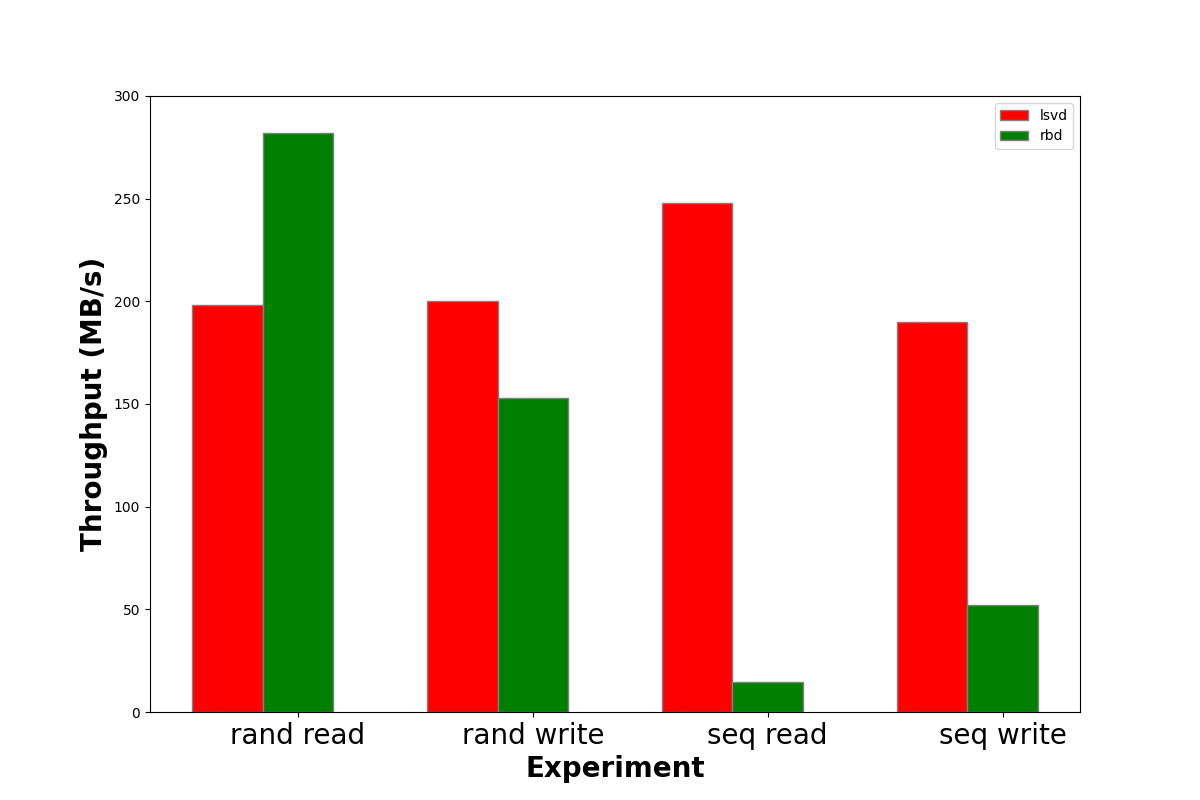
\includegraphics[width=8cm, height=6cm]{graphs/request_bw_ssd_240gb.png}
Fig6. Micro benchmark result with 20GB Cache, 80GB Volume and SSD Backend.

-- more results to be added--







